\documentclass[12pt]{article}
	
\usepackage[margin=1in]{geometry}		% For setting margins
\usepackage{amsmath}				% For Math
\usepackage{fancyhdr}				% For fancy header/footer
\usepackage{graphicx}				% For including figure/image
\usepackage{cancel}					% To use the slash to cancel out stuff in work

%%%%%%%%%%%%%%%%%%%%%%
% Set up fancy header/footer
\pagestyle{fancy}
\fancyhead[LO,L]{Kate O'Neill - 21365768}
\fancyhead[CO,C]{CSU11031 - Electronics Assignment 2}
\fancyhead[RO,R]{\today}
\fancyfoot[LO,L]{}
\fancyfoot[CO,C]{\thepage}
\fancyfoot[RO,R]{}
\renewcommand{\headrulewidth}{0.4pt}
\renewcommand{\footrulewidth}{0.4pt}
%%%%%%%%%%%%%%%%%%%%%%

\begin{document}
\noindent 1.) Connect up the circuit below using Multisim placing the voltmeter and ammeters at the locations shown. The supply voltage is:\\
\[v(t) = 20 \sin (1000 \pi t + \frac{\pi}{4}) V\]\\
(i) Run the simulation. What do you observe? Please provide a superimposed plot of the voltages and currents using Grapher.\\
\begin{figure}[!h] 
	\begin{centering}
		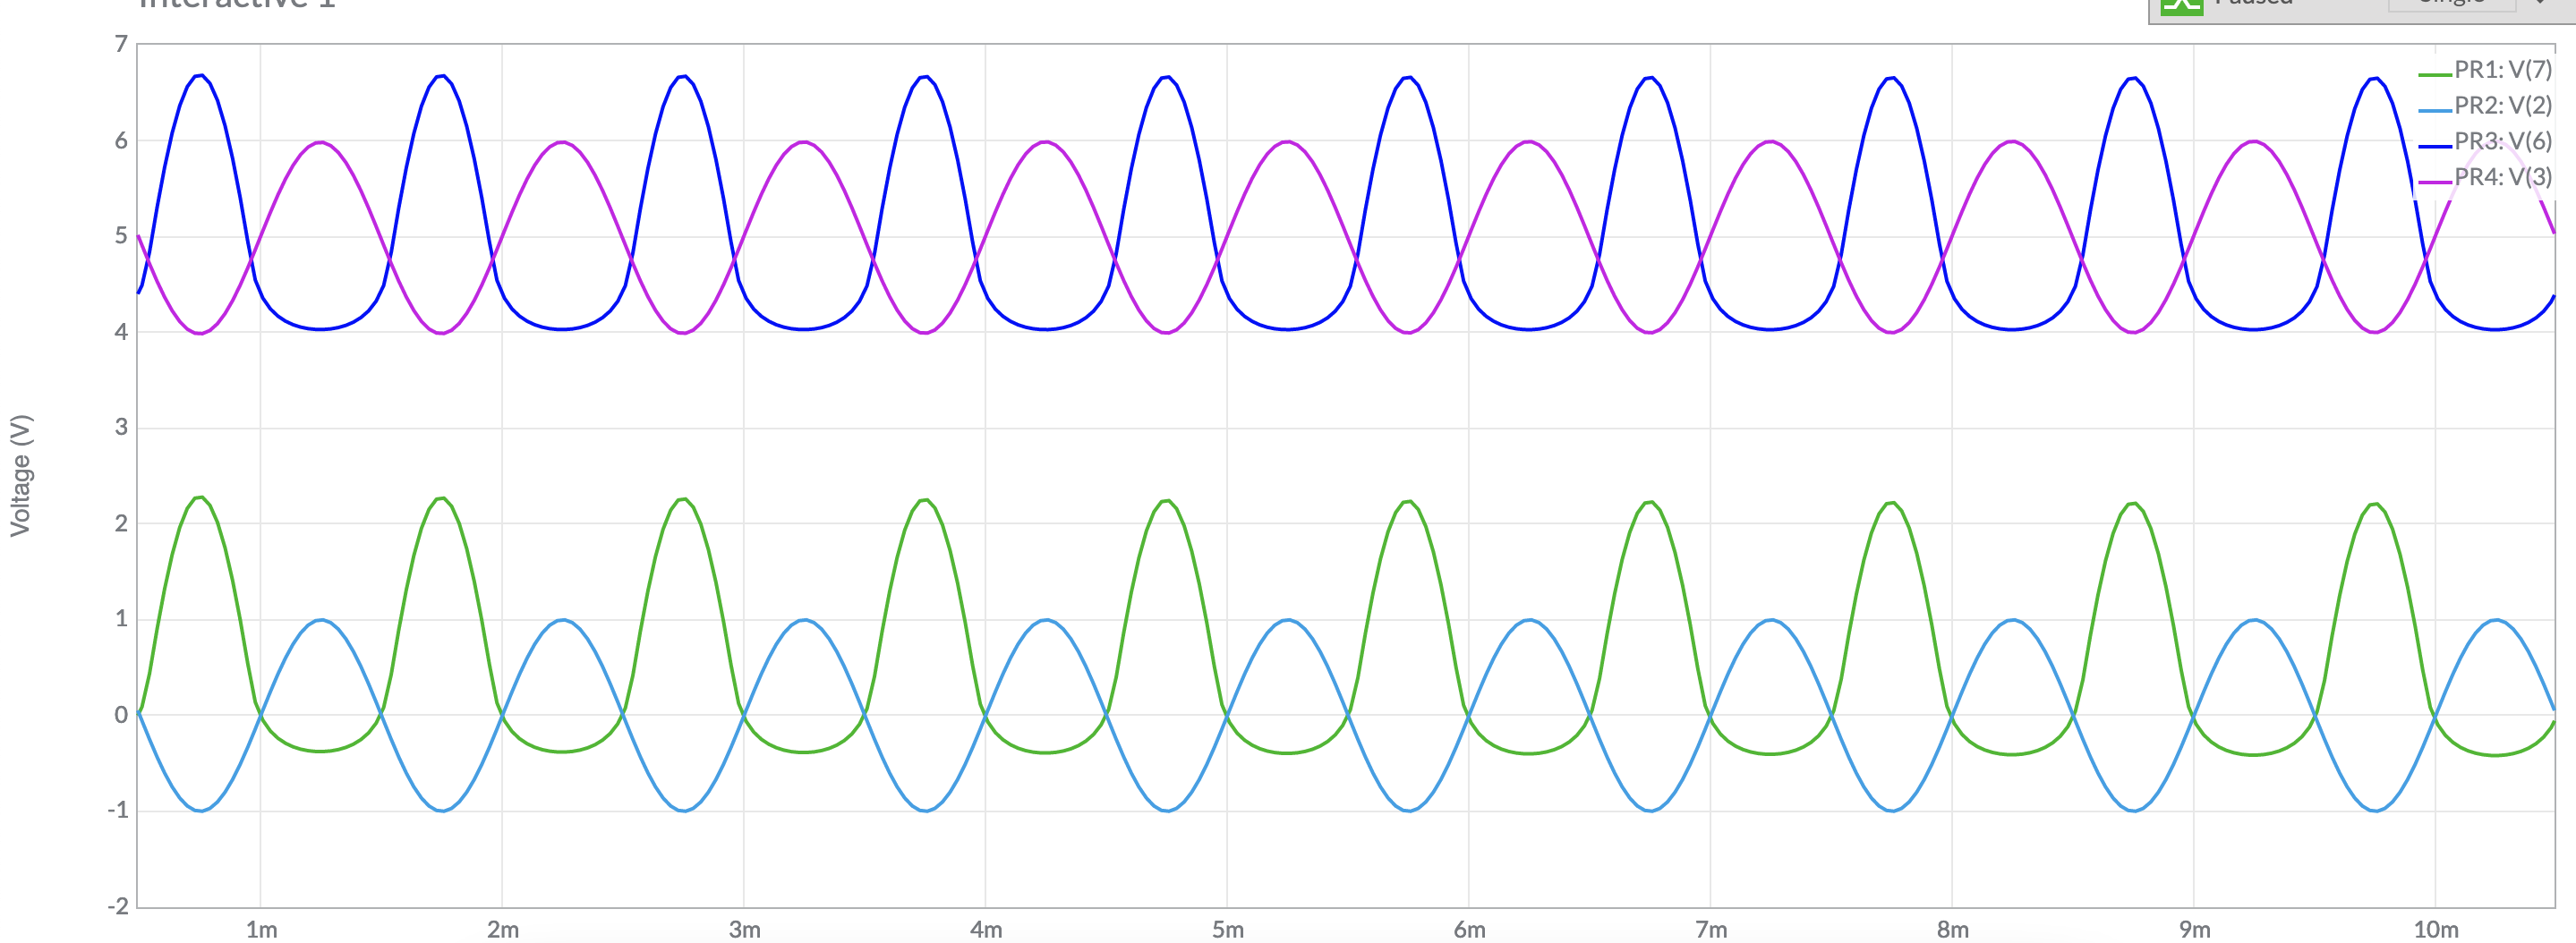
\includegraphics[keepaspectratio = true, width = 6in]{q1(i).PNG}
	\end{centering}
\end{figure}\\
\noindent The 20 in the formula above corresponds to the amplitude in volts of the supply voltage.\\
Upon observation of the voltage value in green on the graph, we can see that at it's peak, it measures 20V and at it's trough, it measures -20V. This is a peak to trough value of 40. Therefore it's amplitude is \(\frac{40}{2}\)V or 20V.\\
This corresponds to the amplitude of 20V of the given function.\\
\\
The \(1000\pi\) in the formula above corresponds to the frequency in radians of the supply voltage.\\
Using \(f = \frac{1}{T}\), where \(f\) is the frequency in Hertz, and \(T\) is the time to complete one cycle in seconds which seems to be approximately 0.002 seconds,\\
\[f = \frac{1}{T}\]
\[f = \frac{1}{0.002}\]
\[f = 500Hz\]\\
Having found the frequency in Hertz, we can now calculate the frequency of the supply voltage in radians using \(\omega = 2 \pi f\), where \(\omega\) is the frequency in radians, and \(f\) is the frequency in Hertz.\\
\[\omega = 2 \pi f\]
\[\omega = 1000 \pi\]\\
This corresponds to the frequency of the given function.\\
\\
The \(\frac{\pi}{4}\) in the formula above corresponds to the phase shift of the supply voltage. this seems the also correspond roughly with the graph.\\
\\
(ii) Calculate the current through the capacitor. Verify your result with the reading from the plot. Why is the supply voltage 90 degrees out of phase with the capacitor current?\\
\\
In order to calculate the current through a capacitor, the formula is \(i(t) = C \frac{dv(t)}{dt}\), where \(C\) is the capacitance of the capacitor in Farads, and \(\frac{dv}{dt}\) is the derivative of the voltage across the capacitor.\\
\\
First, we will find \(\frac{dv}{dt}\) by differentiating \(v(t)\).\\
\[\frac{dv}{dt}[20 \sin (1000\pi t + \frac{\pi}{4})]\]
\[= 20\frac{dv}{dt}[\sin(1000\pi t + \frac{\pi}{4})]\]
\[= 20\cos (1000\pi t + \frac{\pi}{4})(1000\pi)\]
\[= 20000\pi t \cos (1000\pi t + \frac{\pi}{4})\]\\
Now we can find the current through the capacitor with \(i(t) = C \frac{dv(t)}{dt}\).\\
\[i(t) = 50 \times 10^{-6}[20000\pi \cos (1000\pi t + \frac{\pi}{4})]\]
\[i(t) = \pi \cos (1000\pi t + \frac{\pi}{4} )\]\\
\newpage
In order to verify this, we shall substitute t with values from the graph.\\
\begin{figure}[!h] 
	\begin{centering}
		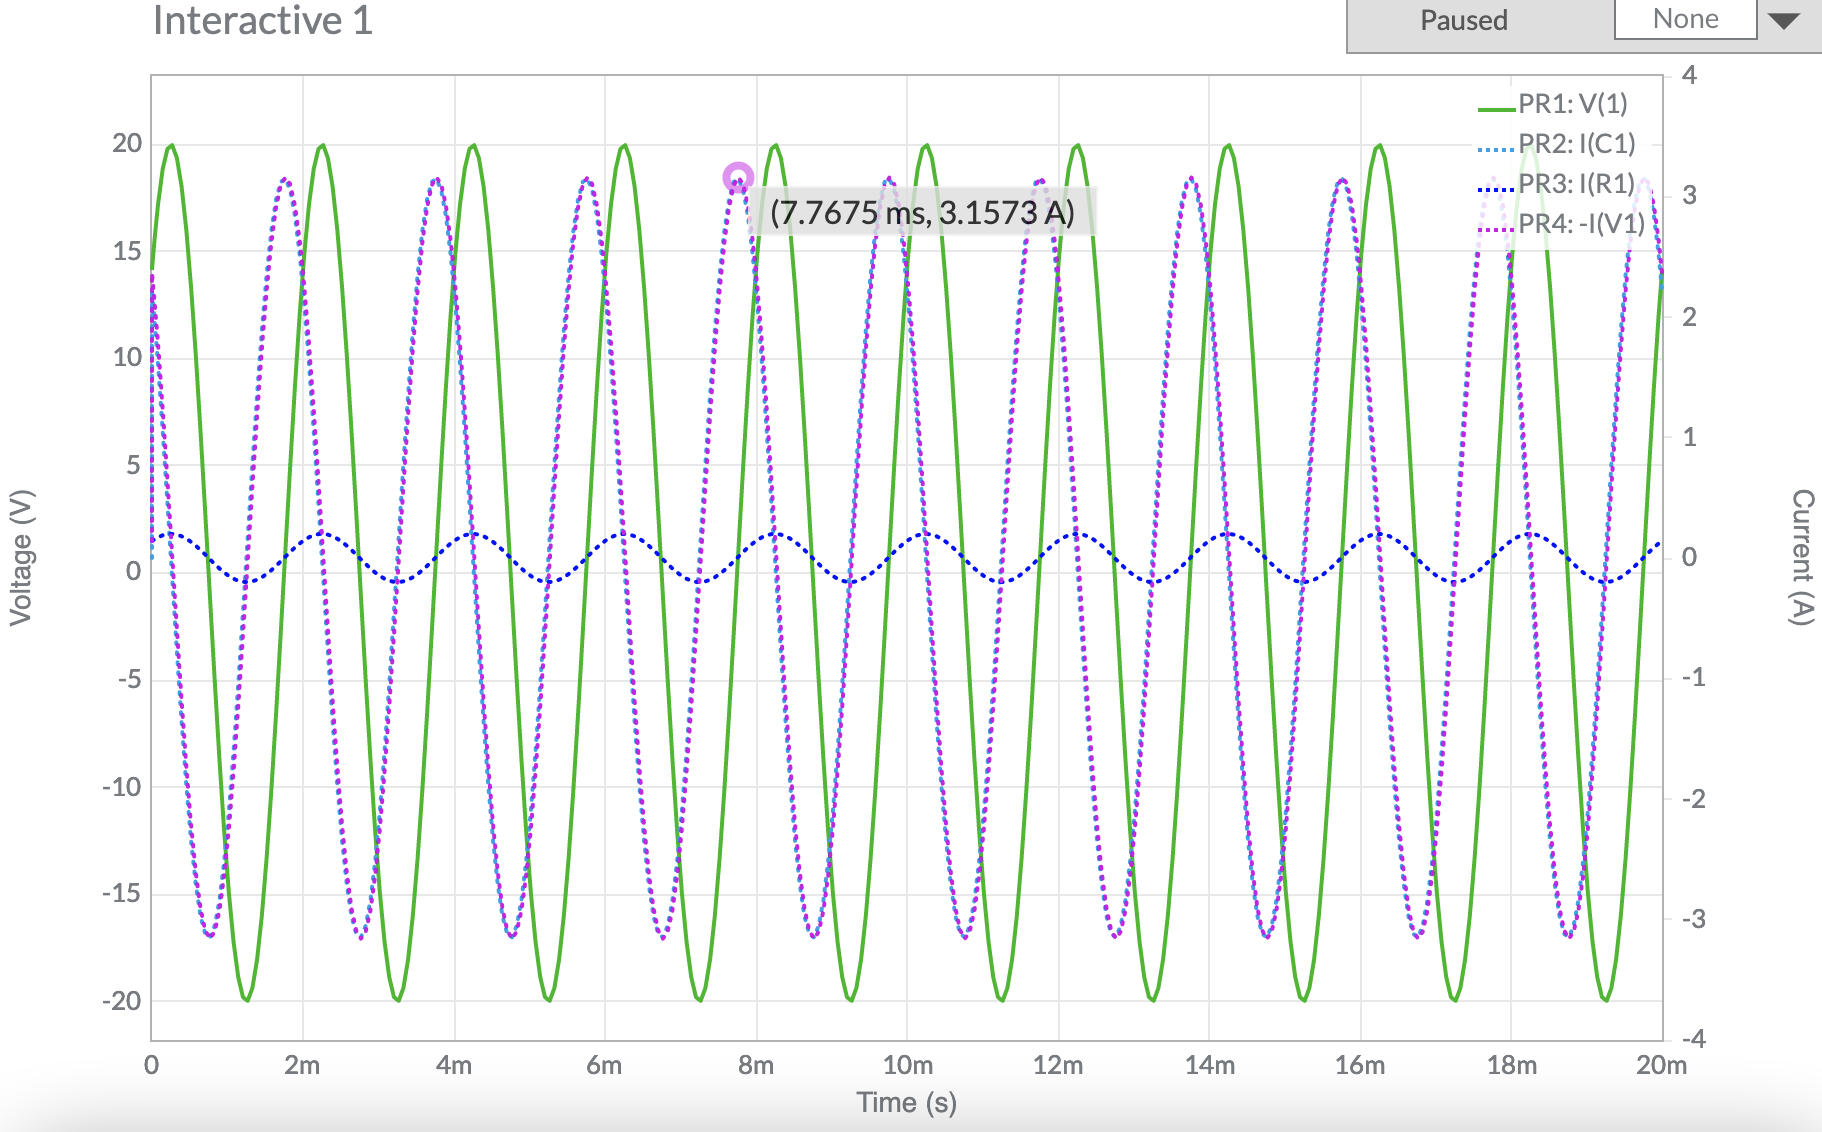
\includegraphics[keepaspectratio = true, width = 6in]{q1(ii).png}
	\end{centering}
\end{figure}\\
\noindent Substituting \(t\) for \(7.7675 \times 10^{-3}\), we get\\
\[I = \pi \cos [1000 \pi (7.7675 \times 10^{-3})]\]
\[= 2.8429 A\]\\
This isn't the exact value found on the graph, which is 3.1573A, but it is quite close. This could be due to a rounding error.\\
\\
Capacitors require a small amount of time to charge before creating any output. Therefore it reaches its peak some time after the voltage. This is why the supply voltage is 90° out of phase with the capacitor current.\\
\\
(iii) Calculate the total current drawn from the source. Compare with the result given by the simulator.\\
\\
Total current in a parallel circuit is equal to the sum of the individual branch currents.\\
\[I_{Total}  = I_1 + I_2 + ... + I_n\]
\[I_{Total} = I_{Resistor} + I_{Capacitor}\]\\
Using Ohm's Law to calculate \(I_{Resistor}\),\\
\[V_{Resistor} = I_{Resistor} R_{Resistor}\]
\[20\cos (1000\pi t + \frac{\pi}{4}) = I_{Resistor}(100)\]
\[I_{Resistor} = \frac{20\cos (1000\pi t + \frac{\pi}{4})}{100}\]
\[= 0.2\cos (1000\pi t + \frac{\pi}{4})\]\\
Having already found \(I_{Capacitor}\) in part (ii),\\
\[I_{Capacitor} = \pi \cos (\pi t + \frac{\pi}{4})\]
\[I_{Total} = 0.2\cos (1000\pi t + \frac{\pi}{4})\]
\[= \cos (1000\pi t + \frac{\pi}{4})(\pi + 0.2)\]\\
In order to verify this, we shall substitute \(t\) with values from the graph.\\
\begin{figure}[!h] 
	\begin{centering}
		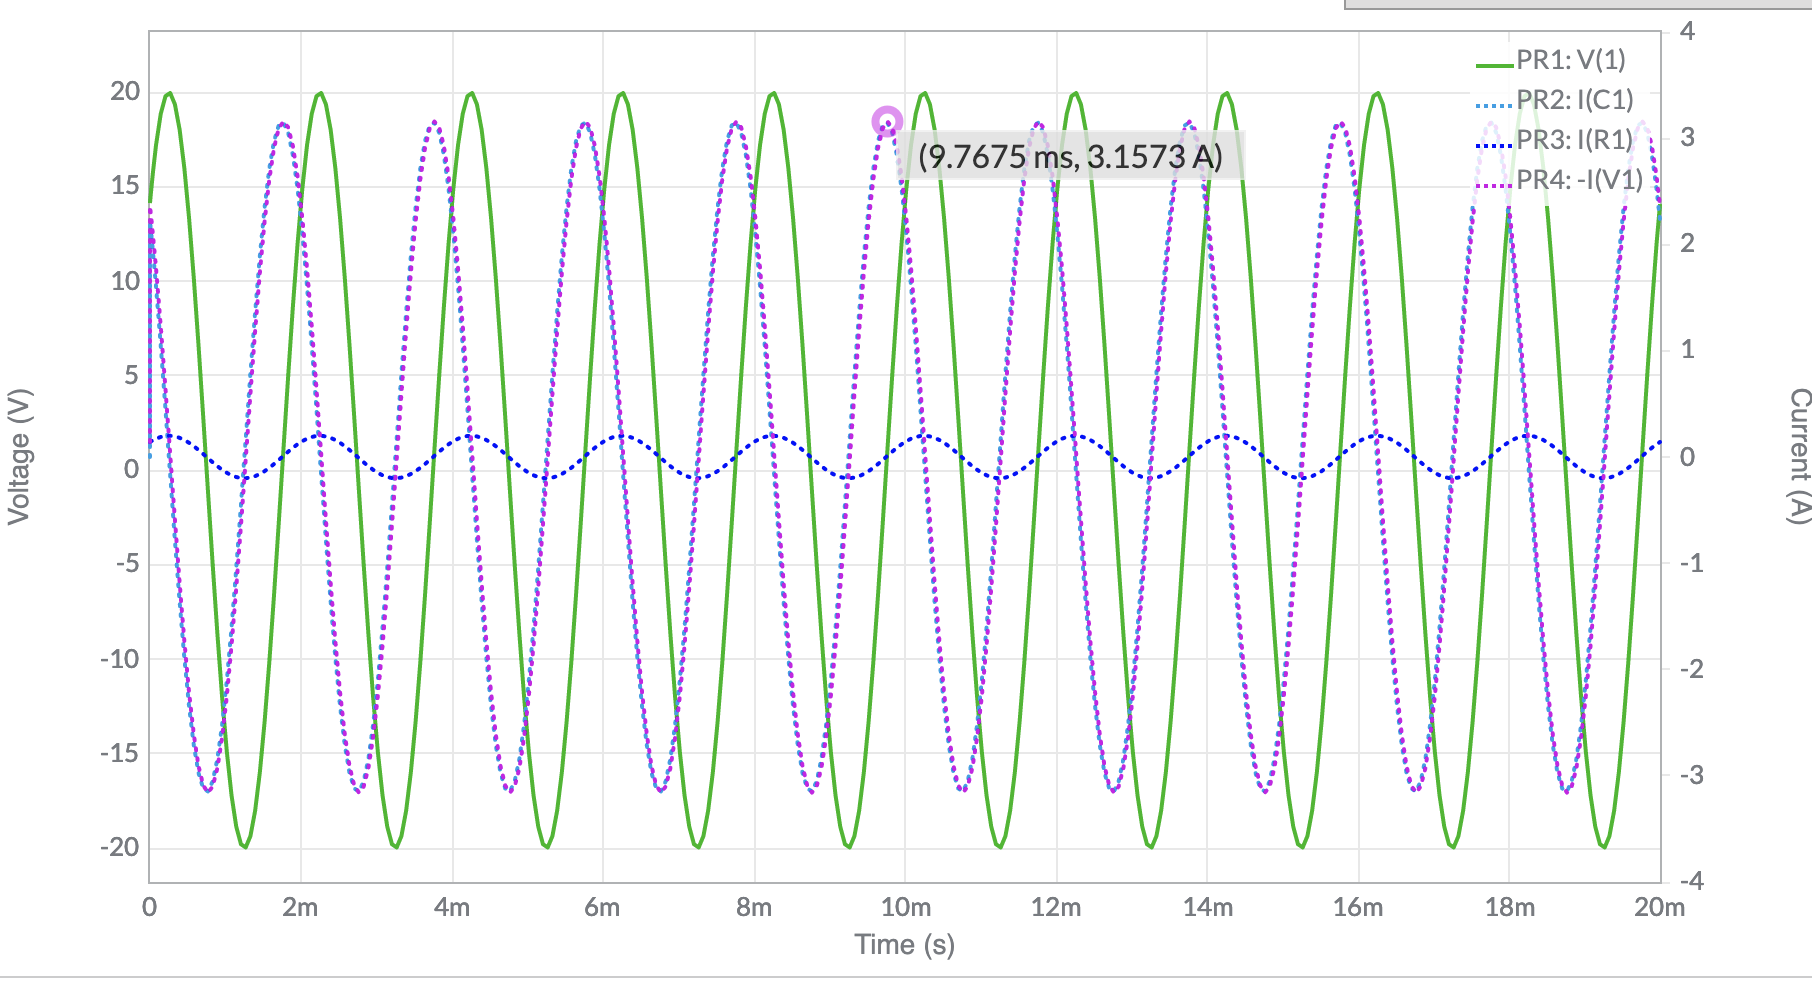
\includegraphics[keepaspectratio = true, width = 6in]{q1(iii).png}
	\end{centering}
\end{figure}\\
Substituting \(t\) for \(9.7675 \times 10^{-3}\), we get\\
\[I = \cos (1000\pi t + \frac{\pi}{4})(\pi + 0.2)\]
\[I = \cos (1000\pi (9.7675 \times 10^{-3}) + \frac{\pi}{4})(\pi + 0.02)\]
\[I = 2.8501A\]\\
This isn't the exact value found on the graph, which is \(3.1573A\), but it is quite close. This could be due to a rounding error.\\
\\
2.) Connect up online the circuit below using Multisim:\\
Place voltmeters and an ammeter at the locations indicated. The supply current is:\\
\[i(t) = 5 \sin (1000\pi t + \frac{\pi}{3})A\]\\
Run the simulation.\\
\\
(i) Calculate the voltage across the inductor. Verify your result by observing this voltage on Grapher. Why is the inductor voltage out of phase by approximately 90 degrees with the load (or supply) voltage?\\
\\
In order to calculate the voltage across an inductor, the formula is \(V_L(t) = L \times \frac{di(t)}{dt}\), where L is the inductance of the inductor in Henrys, and \(\frac{di}{dt}\) is the derivative of the current across the inductor.\\
First, we will find \(\frac{di}{dt}\) by differentiating \(i(t)\).\\
\[\frac{di}{dt}[5\sin (1000\pi t + \frac{\pi}{3})]\]
\[=5 \frac{di}{dt}[\sin (1000\pi t + \frac{\pi}{3})]\]
\[=5 \cos (1000\pi t + \frac{\pi}{3})(1000\pi)\]
\[=5000\pi \cos(1000\pi t + \frac{\pi}{3})\]\\
Now we can find the voltage across the inductor with \(V_L(t) = L \times \frac{di(t)}{dt}\).\\
\[V_L(t) = L \times \frac{di(t)}{dt}\]
\[V_L(t) = (10 \times 10^{-3})[50\pi \cos (1000 \pi t + \frac{\pi}{3})]\]
\[V_L(t) = 50\pi \cos (1000 \pi t + \frac{\pi}{3})\]\\
\newpage
In order to verify this, we shall substitute \(t\) with values from the graph.\\
\begin{figure}[!h] 
	\begin{centering}
		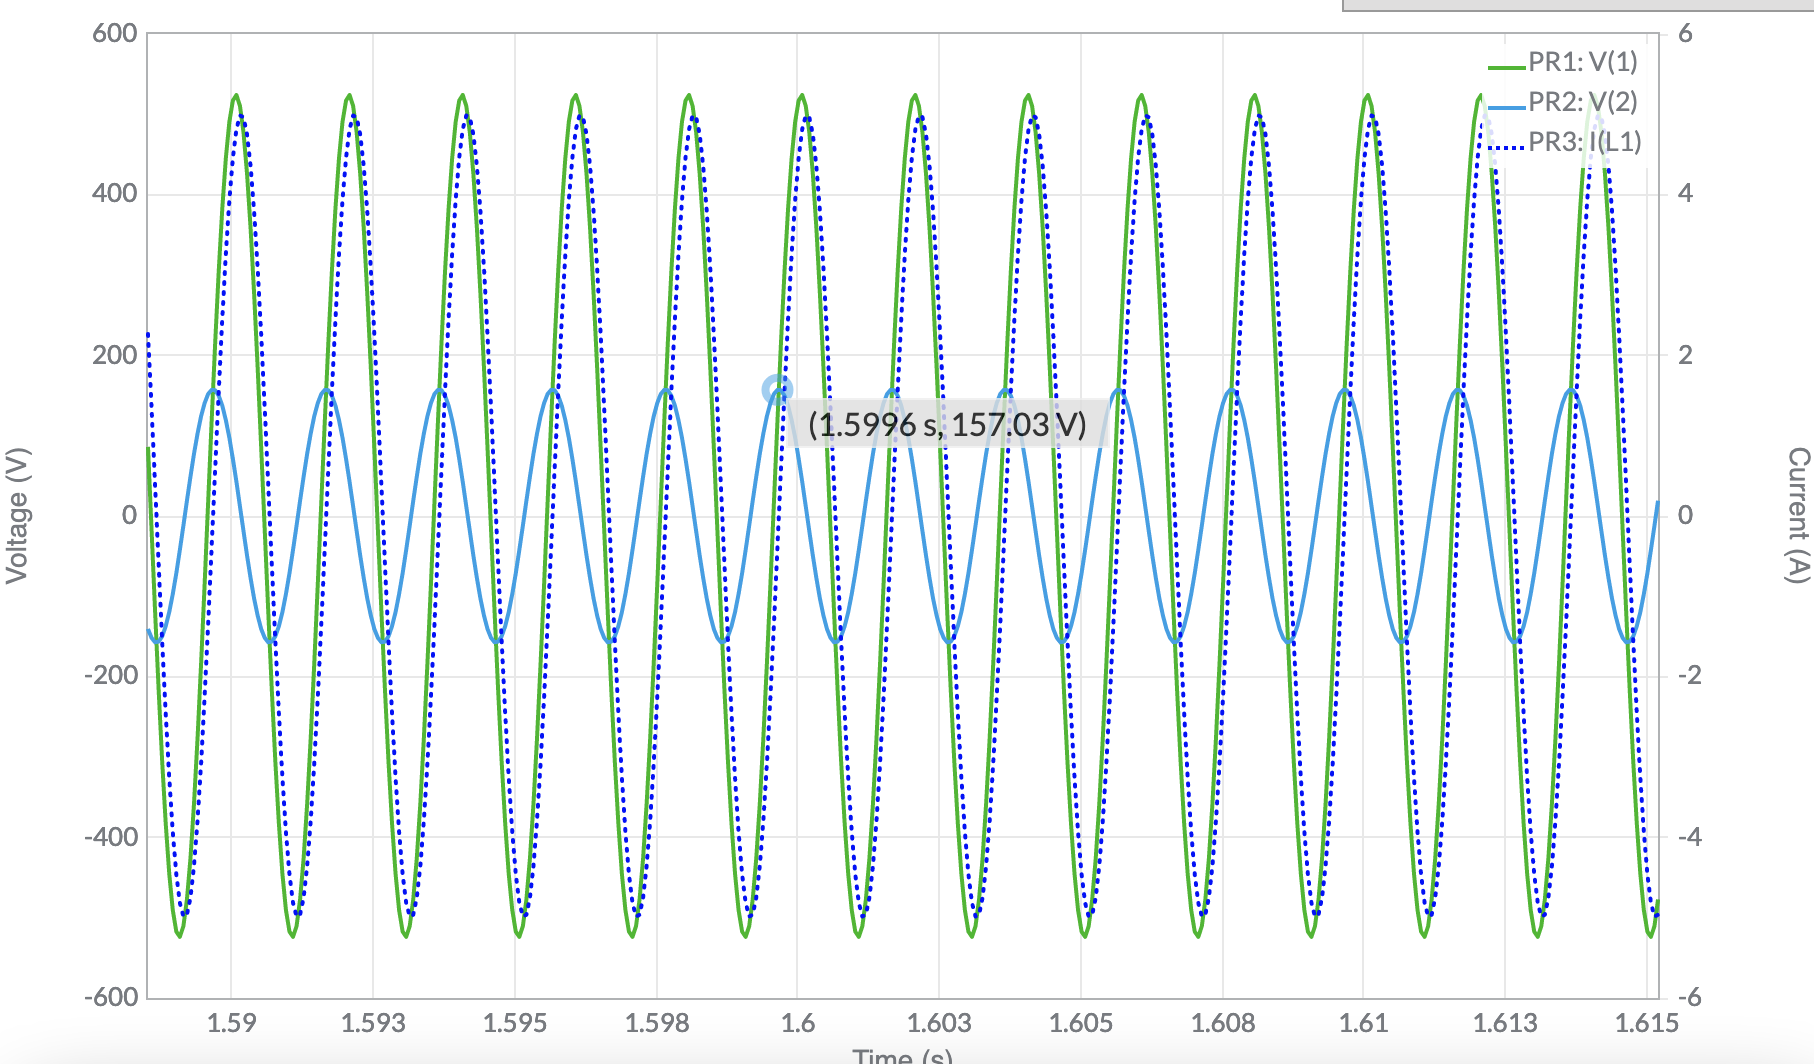
\includegraphics[keepaspectratio = true, width = 6in]{q2(i).png}
	\end{centering}
\end{figure}\\
\noindent Substituting \(t\) for 1.5996, we get\\
\[V = 50 \pi \cos (1000\pi t + \frac{\pi}{3})\]
\[V = 50\pi \cos (1000\pi (1.5996) + \frac{\pi}{3})\]
\[V = 152.6357 V\]\\
This isn't the exact value found on the graph, which is \(157.03V\), but it is quite close. This could be due to a rounding error.\\
\\
When A.C. voltage is applied to an inductor, back emf is produced. It limits the current through the inductor therefore the current lags behind the voltage by 90°.\\
\\
(ii) Calculate the total voltage across the load (resistor-inductor combination). Verify (approximately) your result by observing this voltage on Grapher.\\
\\
Using Ohm's Law, we shall first calculate the voltage through the resistor\\
\[V_{Resistor} = I_{Resistor}R_{Resistor}\]
\[V_{Resistor} = 50\pi \cos (1000\pi + \frac{\pi}{3}) + 500\sin(1000\pi + \frac{\pi}{3})\]\\
The total voltage across the load is equal to the sum of the voltage across the inductor and the voltage across the resistor.\\
\[V_{Total} = V_{Inductor} + V_{Resistor}\]
\[V_{Total} = 50\pi \cos (1000\pi t + \frac{\pi}{3}) + 500\sin (1000\pi t + \frac{\pi}{3})\]\\
In order to verify this, we shall substitute \(t\) with values from the graph.\\
\begin{figure}[!h] 
	\begin{centering}
		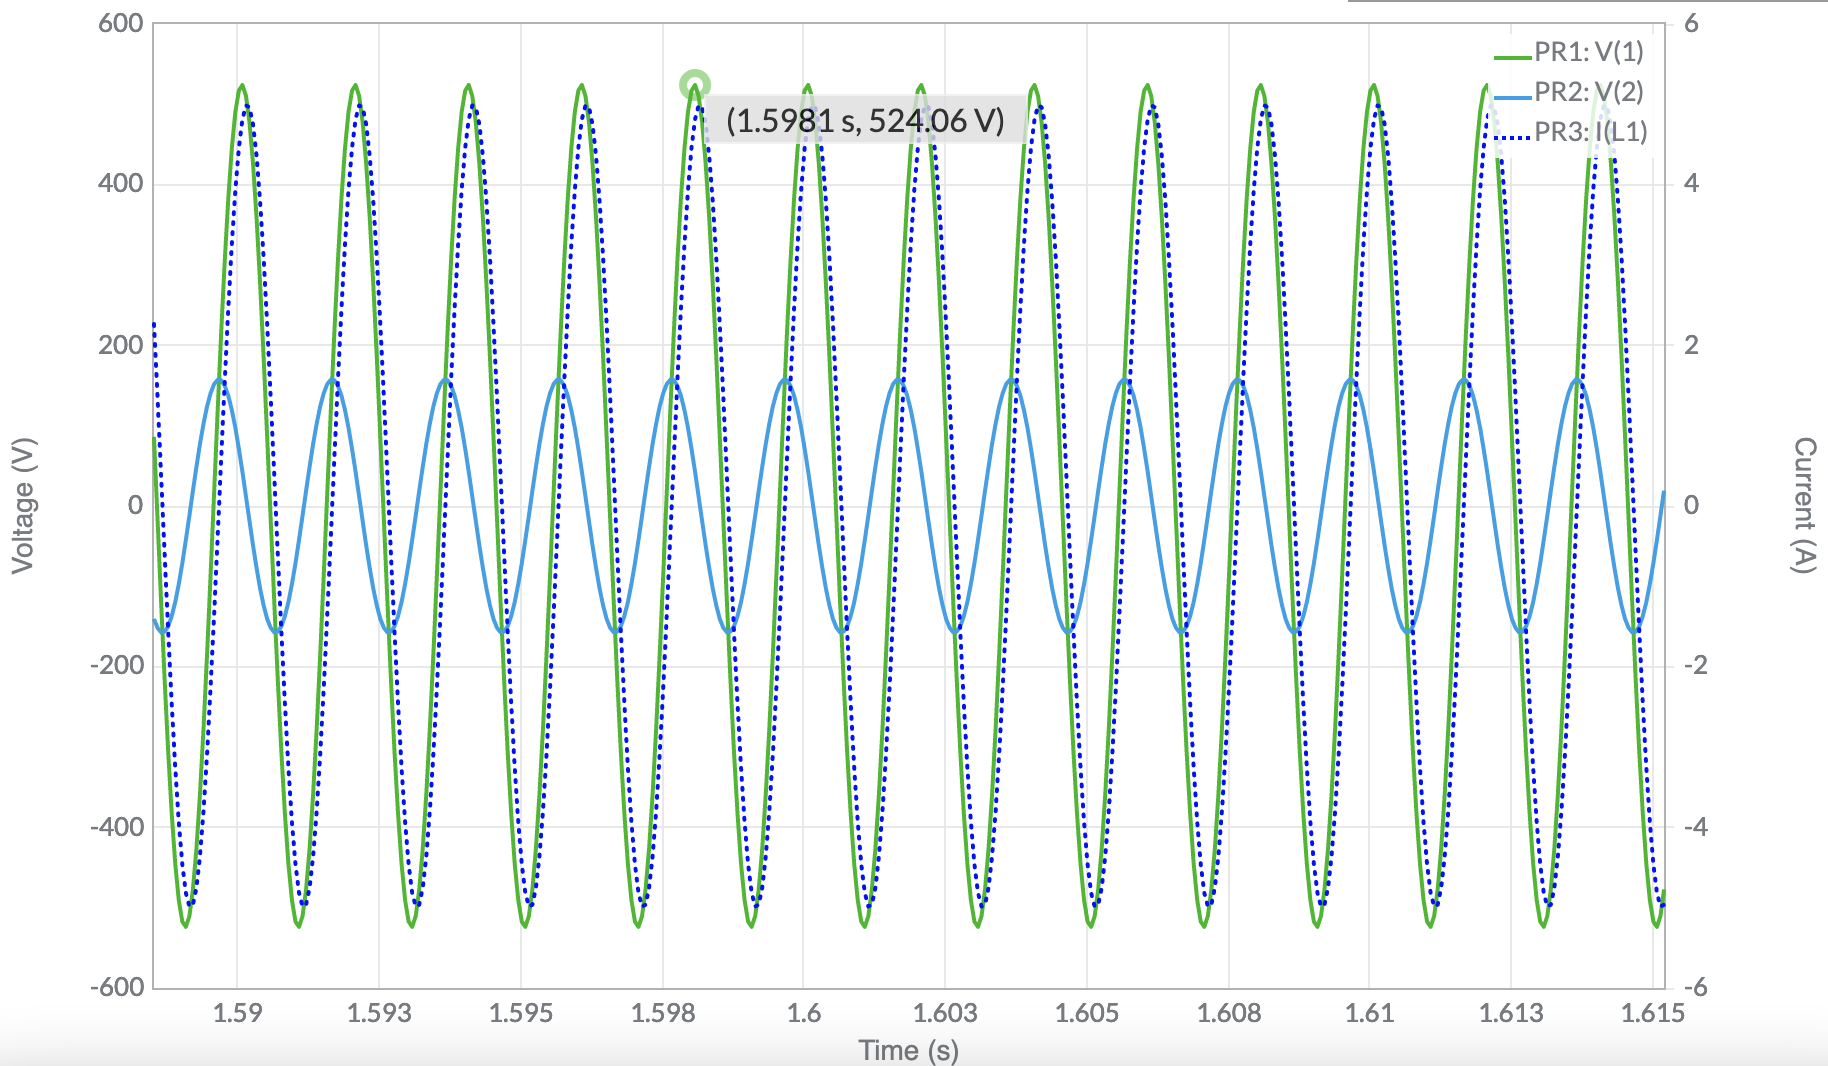
\includegraphics[keepaspectratio = true, width = 6in]{q2(ii).png}
	\end{centering}
\end{figure}\\
\noindent Substituting \(t\) for 1.5981, we get\\
\[V = 50\pi \cos(1000\pi (1.5981) + \frac{\pi}{3}) + 500 \sin(1000\pi (1.5981) + \frac{\pi}{3})\]
\[V = -8.5338V\]\\
This is very different to the value found on the graph, which is 524.06V. This must be due to an error on my part.
\end{document}